\section{Introduction}

Since the publication of RT-1 \cite{RT-1} the robotics research is undergoing a prolific period focused around foundation models. The central promise of this paradigm is the development of generalist policies that aim to achieve general-purpose embodied intelligence, capable of complex interactions within unstructured environments. This shift mirrors advancements in Machine Learning, particularly in Natural Language Processing and Computer Vision, where large pretrained models have demonstrated remarkable success.

\begin{wrapfigure}{r}{0.45\textwidth}
    \centering
    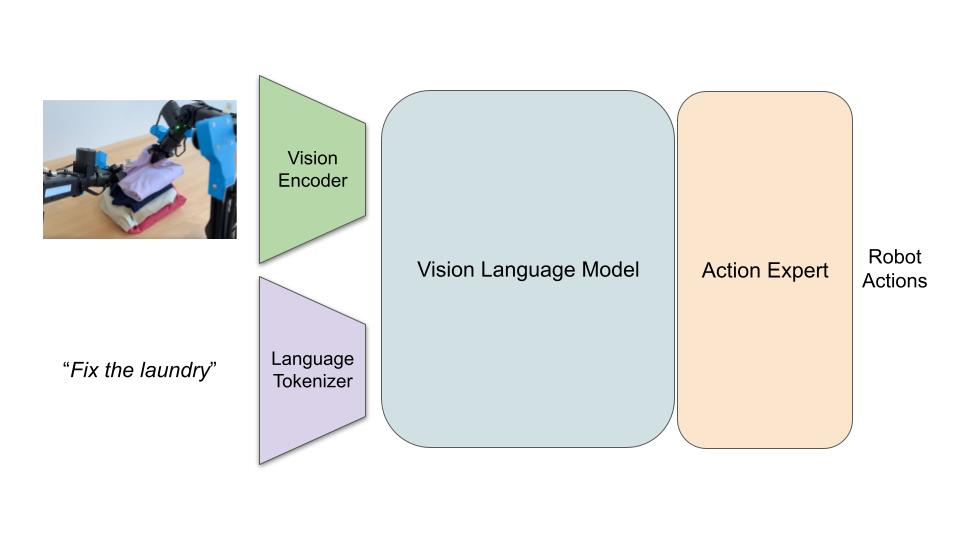
\includegraphics[width=0.45\textwidth]{images/vla.jpg}
    \caption{VLA abstraction}
    \label{fig:vla_abstraction}
    % https://docs.google.com/presentation/d/1F3-KIjQxwBtXfJAlc9_vwuBLSGuZqcXqZ7_GfxX5kYY/edit?usp=sharing
\end{wrapfigure}

Robotics foundational models, often referred to as Vision-Language-Action (VLA) models, is the name of the policies emerging from this paradigm shift. This nomenclature reflects their modality: vision and language for inputs while action as outputs (Figure \ref{fig:vla_abstraction}). Leveraging techniques such as Imitation Learning and Reinforcement Learning, these models demonstrated remarkable capabilities in dexterous manipulation across multiple tasks, offering a degree of generalization over robot embodiments and environments. The key enabler of this progress is the usage of a pretrained vision language model for initialization of the model (or part of the model), and subsequently exploit a vast and variegated robotics dataset to train the Vision Language Action Model.

\section{Goals and Objectives}
Due to the rapid pace of development in robotics foundation models, the field currently lacks established, comprehensive comparison benchmarks, particularly for complex interaction scenarios like deformable object manipulation (DOM). This makes rigorous comparison between proposed models (e.g., $\pi_0$, $Gr00t_{N1}$, $OpenVLA$) challenging. While some models like $\pi_0$ have demonstrated specific DOM tasks (Shirt/Towel/Laundry Folding), a standardized suite is needed for equitable evaluation and deeper understanding.

The primary objective of this project is to develop DOM-Bench: a standardized benchmarking suite tailored for evaluating robotics foundation models on deformable object manipulation tasks. This will provide a coherent and equitable basis for comparing model capabilities and limitations.


\subsection{Overall Goal}

This project aims to deliver:
\begin{itemize}
    \item DOM-Bench Suite: A set of deformable object manipulation tasks, environments, and metrics designed to evaluate robotics foundation models.
    \item Evaluation Protocol and Implementation: Specify the procedure for applying the benchmark suite to different models, e.g: specifications for data efficiency testing and implement the protocol on selected models.
    \item Paper: Summarization of findings, and dissemination through a research paper.
\end{itemize}


\subsection{Specific Objectives}

% To achieve the overall goal, the following specific objectives are defined:

\subsubsection{Literature Review} % Using subsubsection for better structure
The first task is to conduct a comprehensive review covering: existing robotics benchmarks, evaluation methodologies, and taxonomies, with a focus on deformable object manipulation and metrics used; Robotics foundation models (VLAs), detailing architectures, training data/recipes, and claimed capabilities relevant to manipulation.

\subsubsection{Benchmark Design (DOM-Bench)}
Following our review, we will propose DOM-Bench, a benchmark suite and evaluation protocol designed for evaluating robotics foundational models over Deformable Object Manipulation (DOM) tasks. The primary goal of DOM-Bench is to offer deeper insights into a model's capabilities, moving beyond simple task success rates.
To achieve this, DOM-Bench will employ a multi-tier task structure. Tasks are organiyzed into tiers of increasing complexity, with each tier designed to evaluate distinct capabilities using specific, measurable metrics. (A detailed brainstorming of potential tasks can be found in Appendix~\ref{app:task_suite}).
% \begin{enumerate}
%     \item \textit{Fundamentals}: the focus of the first tier is evaluating the shape control and manipulation primitives using classical objects. Classical examples can be Cloth Folding or Rope Straightening.	
%     \item \textit{Complex Interactions}: the aim on this second type of tasks is to test the model capabilities on more sophisticated interaction, multi-step execution, or tool use. 
%     \item \textit{Foundation Model Evaluation}: the final layer of tasks points to evaluating language understanding, reasoning, planning, and generalization capabilities inherent to foundation models when applied to DOM.
% \end{enumerate}

\paragraph{\textbf{Primitive DOM manipulation} (Minimum Requirement)}

The first result is to gather performance over a series of simple tasks (Appendix~\ref{app:task_suite_1}) whose aim is to evaluate the core deformable object manipulation abilities of the models.

\begin{quote} % Or use \hspace*{1em} followed by \parbox{\dimexpr\linewidth-1em\relax}{...} for manual indent
    \textbf{Example} Picking a task for each type of deformable object (rope 1D, fabric 2D and liquid 3D) from the DaXBench simulator - \{WhipRope, FoldTShirt, PourSoup\}. This test will cover a single environment, and a single embodiment (since the DaXBench provides end effector control), therefore we will need to generate forward and inverse kinematics for coherence with the output of the models.
\end{quote}



\paragraph{\textbf{Evaluating Data Efficiency} (Minimum Requirement) }

Beyond task performance, a key aspect of DOM-Bench is the measurement of data efficiency. We aim to quantify how model performance changes based on the amount of fine-tuning data provided. Specifically, we plan to record performance under different conditions: zero-shot (no fine-tuning examples), fine-tuned with 10 examples, fine-tuned with 30 examples.

\begin{quote}
    \textbf{Example} Consider evaluating a Vision-Language-Action (VLA) model on a set of tasks: \{HangClothes, StoreInCloset, PourRice\}. Where HangClothes and StoreInCloset are defined in GarmentLab (a simulated environment, with a specific embodiment), while PourRice will be executed in the RPL lab (a real environment, where we can test different embodiment, e.g., SO-100 and +1 from RPL). To measure data efficiency comprehensively, we need to aggregate performance across these variations. For a single VLA model, the total number of tests required would be calculated based on the variations per task: 1 (HangClothes) + 1 (StoreInCloset) + 2 (PourRice, one for embodiment) = 4 variations. And finally each variation will be tested under 3 different data conditions \{ \text{0-shot, 10 demos, 30 demos} \} resulting in 12 tests.
\end{quote}

% \textbf{Total Variations:} 1 (HangClothes) + 1 (StoreInCloset) + 2 (PourRice, one for embodiment) = 4 variations. Considering that each variation needs to be tested under the 3 different data conditions: \{ \text{0-shot, 10 demos, 30 demos} \} the first metric needs 12 tests

% For instance, considering the full scope mentioned in the reference might involve 3 tasks, 2 simulation environments, 1 real environment, and 3 robot embodiments, leading to a more extensive set of tests.

This approach allows for measuring generalization across tasks, environments (simulation and real), and robot embodiments, similar to the methodology in \cite{TransferWelle}.

\paragraph{\textbf{Further Tasks Expansion} (Stretch Goal) } Include more tasks to each evaluation metric.

\paragraph{\textbf{Context Horizon Quantification} (Stretch Goal)} Design specific long-horizon tasks (picking from Appendix~\ref{app:task_suite_3}) to quantitatively assess the effective context length a model can utilize for successful task completion with DOM. This involves evaluating performance degradation as task complexity and required memory increase.


\paragraph{\textbf{Explainable AI Integration} (Stretch Goal) } Incorporate methods (e.g., representational probing \cite{Probing-VLA}, attention analysis) to gain insights into the models' internal representations and decision-making processes during DOM tasks. This aims to move beyond black-box evaluation towards understanding \textit{why} models succeed or fail.

% \paragraph{Protocol Definition:} Define a precise experimental protocol specifying setup, initial state randomization, number of trials, permissible interventions (if any), and data logging requirements. Reference Appendix \ref{app:task_suite} for detailed task specifications.

\subsubsection{Evaluation \& Analysis}
Implement the defined evaluation protocol using the DOM-Bench suit. Therefore, the first step is to apply the protocol to a core set of publicly available foundation models:
\begin{itemize}
    \item $\pi_0$ \cite{pi_zero}
    \item OpenVLA \cite{OpenVLA}
    \item Gr00t N1 \cite{Gr00tN1}
\end{itemize}
And a posteriori, analyze the results based on the defined metrics, focusing on comparative performance across models, tiers, generalization axes, and data efficiency levels.

\paragraph{Stretch Goals:}


Evaluation expansion can be achieved by adding additional models:
    \begin{itemize}
        \item OpenVLA-OFT \cite{OpenVLA-OFT}
        \item Octo \cite{Octo}
    \end{itemize}
Or by conducting a deeper analysis following the extension of the benchmark.


